\documentclass[12pt]{article}

\usepackage{sbc-template}
\usepackage{graphicx,url}
\usepackage[utf8]{inputenc}
\usepackage[brazil]{babel}
\usepackage[latin1]{inputenc}  

     
\sloppy

\title{Seleção de meta-features e seu efeito na performance de sistemas de meta-aprendizagem}

\author{João Pedro Nunes Magalhães\inst{1}, Victor Hugo Silva Ângelo\inst{1}}


\address{Instituto de Computação (IC) -- Universidade Federal de Alagoas (UFAL)\\
  Av. Lourival Melo Mota, S/N -- Tabuleiro do Martins -- 57072-900 -- Maceió -- AL -- Brazil
  \email{\{jpnm,vsha\}@ic.ufal.br}
}

\begin{document} 

\maketitle

\section{Introdução}

Medir a performance de um sistema de meta-aprendizagem \cite{vanschoren2018meta} vai além de treinar um modelo de aprendizado em meta features, devido a isso, a importancia de selecionar os atributos corretos para construção de meta modelo é a etapa inicial para treinar os modelos. No contexto mais amplo de Automated Machine Learning (AutoML), a seleção de algoritmos e a otimização em Inteligência Artificial são gargalos práticos constantes \cite{he2021automl}. Isso impacta diretamente no processo final de recomendação de algoritmos de machine learning em determinados datasets, porém bibliotecas que extraem meta features de datasets geram uma quantidade de atributos para representação os datasets como número de linhas, número de coluna, entropia dos atributos, etc. Essa dimensionalidade dos atributos pode prejudicar tanto no treinamento do meta modelo quanto na predição do melhor algoritmo, além de processamento, tempo de treinamento, recursos computacional. Assim, esse artigo tem como objetivo automatizar a seleção das meta features utilizando tecnicas de pesquisa operacional como metodos exatos e metodos aproximados, além de uma abordagem hibrida dos dois metodos, consequentemente a recomendação do pipeline para treinamento do sistema de meta-aprendizagem. Além disso, o estudo busca trazer estatisticas como tempo de processamento para selecionar os atributos, performance dos meta modelos, representividade dos atributos selecionados nos modelos, acuracias dos algoritmos de machine learning em nível meta e nível base.


\section{Proposta}

Por estar lidando com problemas de dimensionalidade, de alto custo computacional de extração, de sobreposição informacional, de correlação dos dados, buscou-se forcar principalmente na diminuição das meta features com técnicas exatas e técnicas aproximadas da área de pesquisa operacional. Devido a isso, o problema é categorizado como de combinação e de otimização, em que ao tentar maximizar acurácia, existe uma combinação de atributos de caracteristica dos datasets e verificar todas as combinações possíveis dos atributos é inviável computacionalmente. Em contrapartida às tendências mais recentes de Auto-ML que utilizam arquiteturas neurais complexas para extrair representações e recomendar algoritmos diretamente dos dados, evitando a engenharia de atributos tradicional \cite{wang2023onestep}, a proposta desse estudo é focar na seleção rigorosa das melhores meta features extraídas pela biblioteca pymfe utilizando a função MFE, maximizando o nível de acerto do melhor algoritmo de Machine Leaning para um determinado dataset. Além disso, foi verificado 6 algoritmos aprendizado de máquina (SVM, KNN, Naives Bayes, DecisionTree, RandomForest, ExtraTreesClassifier) durante o estudo para entender o impacto que cada um teve durante o processo de treinamento e teste do meta modelo.

\subsection{Metodos Exatos} \label{sub:exato}

Ao categorizar o problema como a escolha das melhores meta features, pode-se adaptar o problema para outros tipos que já possui modelagens matematicas na literura como Problema de Seleção do Melhor Subconjunto, Problema da Mochila com Penalidades e Problema da Mochila Quadrática. Logo, todos essas modelagens precisam de utilizam o calculo da importancia  de cada meta features com a biblioteca sklearn para os modelos que serão treinados para penalizar os modelos, segue os modelos com a técnica respectivimente:

\begin{enumerate}
    \item \textbf{Decision Tree:} Atributo nativo \texttt{feature\_importances\_} (baseado em Redução Média de Impureza - MDI).

    \item \textbf{Random Forest:} Atributo nativo \texttt{feature\_importances\_} (baseado em Redução Média de Impureza do comité).

    \item \textbf{Gaussian Naive Bayes:} Abordagem de filtro estatístico utilizando o valor $F$ da ANOVA via \texttt{f\_classif}.

    \item \textbf{Support Vector Machine (SVM):} Método pós-processamento agnóstico via Importância por Permutação (\texttt{permutation\_importance}).

    \item \textbf{K-Nearest Neighbors (KNN):} Método pós-processamento agnóstico via Importância por Permutação (\texttt{permutation\_importance}).
\end{enumerate}

Por fim, os subtopicos com as modelagens matematicas serão implementadas com a biblioteca Pulp do Python. Essa biblioteca tem como objetivo modelar o problema na linguagem matemática e o solver COIN-OR Branch and Cut (CBC) busca uma solução otima com algum algoritmo (caixa preta). Esses algoritmos tem como caracteristica está na área da Programação Linear Inteira ou Programação Linear Inteira Mista.

\subsubsection{Problema de Seleção do Melhor Subconjunto}

O primeiro método consiste em uma formulação clássica de seleção de atributos com restrição de igualdade estrita. Para um metamodelo específico $m$, o problema de programação linear inteira mista é modelado conforme segue:

\begin{equation} \label{eq:obj_subset}
\text{Maximizar } \quad Z_1 = \sum_{i=1}^{N} S_{m,i} \cdot x_i
\end{equation}

Sujeito a:
\begin{equation} \label{eq:rest_subset}
\sum_{i=1}^{N} x_i = K
\end{equation}

\begin{equation}
x_i \in \{0, 1\}, \quad \forall i \in \{1, \dots, N\}
\end{equation}

\noindent \textbf{Onde:}
\begin{itemize}
    \itemsep0em
    \item $N$: Número total de meta-features candidatas;
    \item $S_{m,i}$: Coeficiente de importância da meta-feature $i$ para o metamodelo $m$;
    \item $K$: Limite máximo e exato de cardinalidade do subconjunto (\texttt{max\_feature});
    \item $x_i$: Variável binária de decisão ($1$ se a meta-feature $i$ for selecionada, e $0$ caso contrário).
\end{itemize}


\subsubsection{Problema da Mochila com Penalidades}

O segundo método flexibiliza o tamanho do subconjunto ao alterar a restrição de cardinalidade para uma desigualdade e introduzir um fator de penalização linear $\lambda$, que atua como um limiar de utilidade para a meta-acurácia:

\begin{equation} \label{eq:obj_knapsack}
\text{Maximizar } \quad Z_2 = \sum_{i=1}^{N} (S_{m,i} - \lambda) \cdot x_i
\end{equation}

Sujeito a:
\begin{equation} \label{eq:rest_knapsack}
\sum_{i=1}^{N} x_i \le K
\end{equation}

\begin{equation}
x_i \in \{0, 1\}, \quad \forall i \in \{1, \dots, N\}
\end{equation}

\noindent \textbf{Onde:}
\begin{itemize}
    \itemsep0em
    \item $\lambda$: Hiperparâmetro de penalidade por baixa utilidade marginal (\texttt{l});
    \item $K$: Limite máximo de cardinalidade do subconjunto (agora tratado como um teto flexível);
    \item Os parâmetros $N$, $S_{m,i}$ e a variável de decisão $x_i$ seguem as definições do modelo anterior.
\end{itemize}


\subsubsection{Problema da Mochila Quadrática Linearizada}

Para mitigar os efeitos de multicolinearidade, o terceiro método penaliza a seleção simultânea de pares de características altamente correlacionadas. O problema é linearizado por meio de variáveis artificiais binárias $z_{i,j}$ para o conjunto de alta correlação $\Omega$. A formulação final para cada metamodelo $m$ é descrita por:

\begin{equation} \label{eq:obj_quad}
\text{Maximizar } \quad Z_3 = \sum_{i=1}^{N} S_{m,i} \cdot x_i - \gamma \sum_{(i,j) \in \Omega} C_{i,j} \cdot z_{i,j}
\end{equation}

Sujeito a:
\begin{equation} \label{eq:rest_quad}
\sum_{i=1}^{N} x_i \le K
\end{equation}

\begin{equation} \label{eq:mccormick1}
z_{i,j} \le x_i, \quad \forall (i,j) \in \Omega
\end{equation}

\begin{equation} \label{eq:mccormick2}
z_{i,j} \le x_j, \quad \forall (i,j) \in \Omega
\end{equation}

\begin{equation} \label{eq:mccormick3}
z_{i,j} \ge x_i + x_j - 1, \quad \forall (i,j) \in \Omega
\end{equation}

\begin{equation}
x_i \in \{0, 1\}, \quad \forall i \in \{1, \dots, N\}
\end{equation}

\begin{equation}
z_{i,j} \in \{0, 1\}, \quad \forall (i,j) \in \Omega
\end{equation}

\noindent \textbf{Onde:}
\begin{itemize}
    \itemsep0em
    \item $\gamma$: Peso computado da penalização de redundância na função objetivo (\texttt{gama});
    \item $C_{i,j}$: Correlação absoluta par a par entre as meta-features $i$ e $j$;
    \item $\theta$: Limiar mínimo de correlação crítica (\texttt{corr\_threshold});
    \item $\Omega = \{(i,j) \mid i < j \text{ e } C_{i,j} \ge \theta\}$: Conjunto restrito de pares de meta-features que ultrapassam a correlação crítica $\theta$;
    \item $z_{i,j}$: Variável auxiliar binária ($1$ se $x_i$ e $x_j$ forem selecionadas simultaneamente, e $0$ caso contrário).
\end{itemize}

As equações (\ref{eq:mccormick1}), (\ref{eq:mccormick2}) e (\ref{eq:mccormick3}) representam a linearização exata do produto lógico $x_i \cdot x_j$, garantindo que a penalidade de redundância $C_{i,j}$ seja computada unicamente quando ambas as características forem selecionadas para o espaço de busca meta.

\subsection{Metodo Aproximado}

Neste método, cada indivíduo do algoritmo genético representa uma possível solução para o problema. Essa solução é codificada em um vetor binário, em que cada posição é associada a uma meta-feature. Quando o valor da posição é igual a 1, a meta-feature é selecionada; quando o valor é igual a 0, ela não é selecionada. Assim, cada indivíduo corresponde a um subconjunto diferente de meta-features.

Para avaliar a qualidade de cada indivíduo, foi treinado um meta-modelo utilizando apenas as meta-features selecionadas por aquele indivíduo, A função de fitness levou em consideração a acurácia média obtida na validação cruzada, mas também aplicou penalizações para evitar soluções com muitos atributos ou com desempenho muito instável entre os folds. A função utilizada foi definida como:

\[
fitness(x) = \overline{Acc}(x) - \lambda \left(\frac{|S_x|}{p}\right)^{\alpha} - \beta \sigma_{Acc}(x)
\]

em que \(\overline{Acc}(x)\) representa a acurácia média do indivíduo, \(|S_x|\) é a quantidade de meta-features selecionadas, (p) é o total de meta-features disponíveis após a filtragem inicial, \(\sigma_{Acc}(x)\) representa o desvio-padrão das acurácias na validação cruzada, e \(\lambda\), \(\alpha\) e \(\beta\) são parâmetros usados para controlar as penalizações da função.

Antes da execução dos algoritmos genéticos, foi realizada uma etapa de filtragem das meta-features. Nessa etapa, foram removidos atributos com muitos valores ausentes, atributos constantes ou quase constantes, atributos duplicados e atributos altamente correlacionados. Depois disso, foi aplicado um filtro baseado em Mutual Information, reduzindo o conjunto para as 150 meta-features mais relevantes. Essa filtragem foi importante para diminuir o tamanho do problema e permitir que os algoritmos genéticos trabalhassem em um espaço de busca menor e mais informativo.

Foram testadas três variações de Algoritmo Genético. O primeiro foi o AG clássico binário, utilizado como uma abordagem base para comparação. Nesse caso, a população inicial foi gerada de forma aleatória, o cruzamento foi feito por um ponto e a mutação ocorreu pela inversão de bits. Esse método não utiliza informação prévia sobre a importância das meta-features, sendo útil para observar o comportamento de uma abordagem genética mais simples.

O segundo método foi um AG guiado por Mutual Information com busca local. Diferente do primeiro, esse algoritmo utiliza o ranking de Mutual Information para ajudar na geração de parte da população inicial. Com isso, algumas soluções já começam com meta-features consideradas mais relevantes. Além disso, o método utiliza cruzamento uniforme, mutação com maior tendência para remover atributos e uma etapa de busca local para tentar melhorar as melhores soluções encontradas. A ideia dessa abordagem foi combinar a busca evolutiva com uma informação prévia sobre os atributos.

O terceiro método foi um AG compacto, com foco em gerar soluções menores. Ele também utiliza uma inicialização guiada, mas possui uma estratégia mais forte de controle da quantidade de meta-features selecionadas. Além disso, utiliza uma mutação adaptativa mais esparsa e impõe um limite máximo para o tamanho do subconjunto selecionado. Essa abordagem foi usada para verificar se seria possível manter uma boa acurácia mesmo utilizando uma quantidade menor de meta-features.

De forma geral, os três algoritmos foram definidos para comparar diferentes comportamentos: o primeiro como uma abordagem mais simples e aleatória, o segundo buscando equilibrar desempenho e redução de atributos, e o terceiro priorizando subconjuntos mais compactos.

\subsection{Abordagem Híbrida}

A proposta desta abordagem consiste em utilizar os métodos exatos como um pré-processamento para a seleção de meta-features. As soluções obtidas por essas modelagens matemáticas são então injetadas como indivíduos elite na população inicial do Algoritmo Genético (Seeded GA), combinando a precisão dos métodos exatos com a capacidade de exploração da meta-heurística.

\section{Metodologia experimental}

\subsection{Métodos Exatos}

A metodologia experimental para os métodos exatos inicia-se com a extração das pontuações de importância de cada meta-feature através dos modelos base: Decision Tree, Random Forest, SVM, KNN e Naive Bayes. Destaca-se que o pré-processamento de padronização (StandardScaler) é aplicado exclusivamente aos dados que alimentam os algoritmos SVM, Naive Bayes e KNN. Todos os modelos detalhados na Seção \ref{sub:exato} são treinados e avaliados por meio da validação cruzada Leave-One-Out. O processo gera um conjunto de meta-features selecionadas para cada modelo. Em seguida, realiza-se uma avaliação cruzada testando os 5 classificadores nos 5 conjuntos de meta-features selecionados, totalizando 25 cenários experimentais distintos. O objetivo desta etapa é determinar a combinação ideal de meta-modelo e meta-features que maximize a acurácia preditiva no nível-meta.

\subsection{Métodos Aproximados}

Visando otimizar o tempo de execução e a eficiência da busca, adotaram-se estratégias específicas para a configuração dos Algoritmos Genéticos (AG). Inicialmente, aplicou-se um pré-processamento rigoroso no \textit{meta-dataset} para a exclusão de atributos com alta correlação, constantes ou com excesso de valores nulos. Em seguida, aplicou-se um filtro supervisionado baseado em Informação Mútua (\textit{Mutual Information}), retendo apenas as 150 \textit{meta-features} mais promissoras.
Para o cálculo da função de aptidão (\textit{fitness}), optou-se pela utilização do modelo \textit{ExtraTreesClassifier}, escolhido por sua elevada velocidade de treinamento e robustez. A avaliação interna desse classificador foi realizada por meio de validação cruzada estratificada (\textit{StratifiedKFold}) com $K = 5$.
A evolução das soluções baseou-se em uma população de 80 indivíduos, evoluindo ao longo de 150 gerações. O processo de seleção utilizou um torneio de tamanho 4 e aplicou-se um elitismo que preserva os 4 melhores indivíduos de cada geração. Os operadores genéticos foram configurados com uma taxa de cruzamento de 85\% e uma taxa de mutação adaptativa, iniciando com uma probabilidade de 10\% nas primeiras gerações e decaindo linearmente para 2\% até o fim do processo evolutivo.
A metodologia abrange a avaliação de três configurações distintas do algoritmo aproximativo: (1) AG Clássico Binário, focado na exploração aleatória; (2) AG Guiado com Busca Local, focado no refinamento e estabilidade; e (3) AG Esparso, com o objetivo de encontrar subconjuntos mínimos de \textit{features}. Consequentemente, ao término desta etapa experimental, serão obtidos 3 meta-modelos finais, cada um representando a melhor solução otimizada por sua respectiva variação algorítmica.

\subsection{Abordagem híbrida}

Por fim, na Abordagem híbrida busca combinar a precisão matemática dos métodos exatos com a ampla capacidade de exploração espacial dos algoritmos genéticos. Para atingir esse objetivo, adotou-se a estratégia conhecida como \textit{Seeded GA} (Algoritmo Genético Semeado). Diferentemente de outras rotas semânticas que abordam o problema de recomendação por meio de ontologias e da qualidade dos dados \cite{nayak2022ontological}, a Abordagem Híbrida aqui proposta fundamenta-se estritamente no rigor matemático da Pesquisa Operacional e na exploração meta-heurística.
Diferentemente da inicialização adotada nos métodos aproximados puros que ocorre de forma estocástica ou guiada por filtros, a população inicial da abordagem híbrida é construída a partir dos resultados obtidos na etapa exata. Especificamente, os melhores subconjuntos de \textit{meta-features} identificados pelas modelagens de Programação Linear Inteira (detalhadas na subseção anterior) são injetados diretamente como indivíduos na população inicial do algoritmo genético.
Para garantir a consistência e a comparabilidade experimental, o algoritmo genético desta fase herda integralmente os hiperparâmetros evolutivos (tamanho da população, taxas de mutação e cruzamento, modelo \textit{ExtraTreesClassifier}) e o rigoroso \textit{pipeline} de pré-processamento já estipulados para os métodos aproximados. Dessa forma, a meta-heurística inicia seu processo evolutivo em regiões do espaço de busca previamente otimizadas pelos métodos exatos, visando refinar as soluções, escapar de eventuais ótimos locais e encontrar a combinação definitiva de \textit{meta-features} para a recomendação de algoritmos.

\section{Resultados e Discussão}

\subsection{Métodos Exatos}

Ao analisar os resultados dos métodos exatos tem-se que o melhor classificador desempenhado foi a DecisionTree. Entretanto, o SVM conseguiu ter uma menor variância em relação aos outros algoritmos, como mostra a Figura~\ref{fig:boxplots_exatos}.

\begin{figure}[ht]
\centering
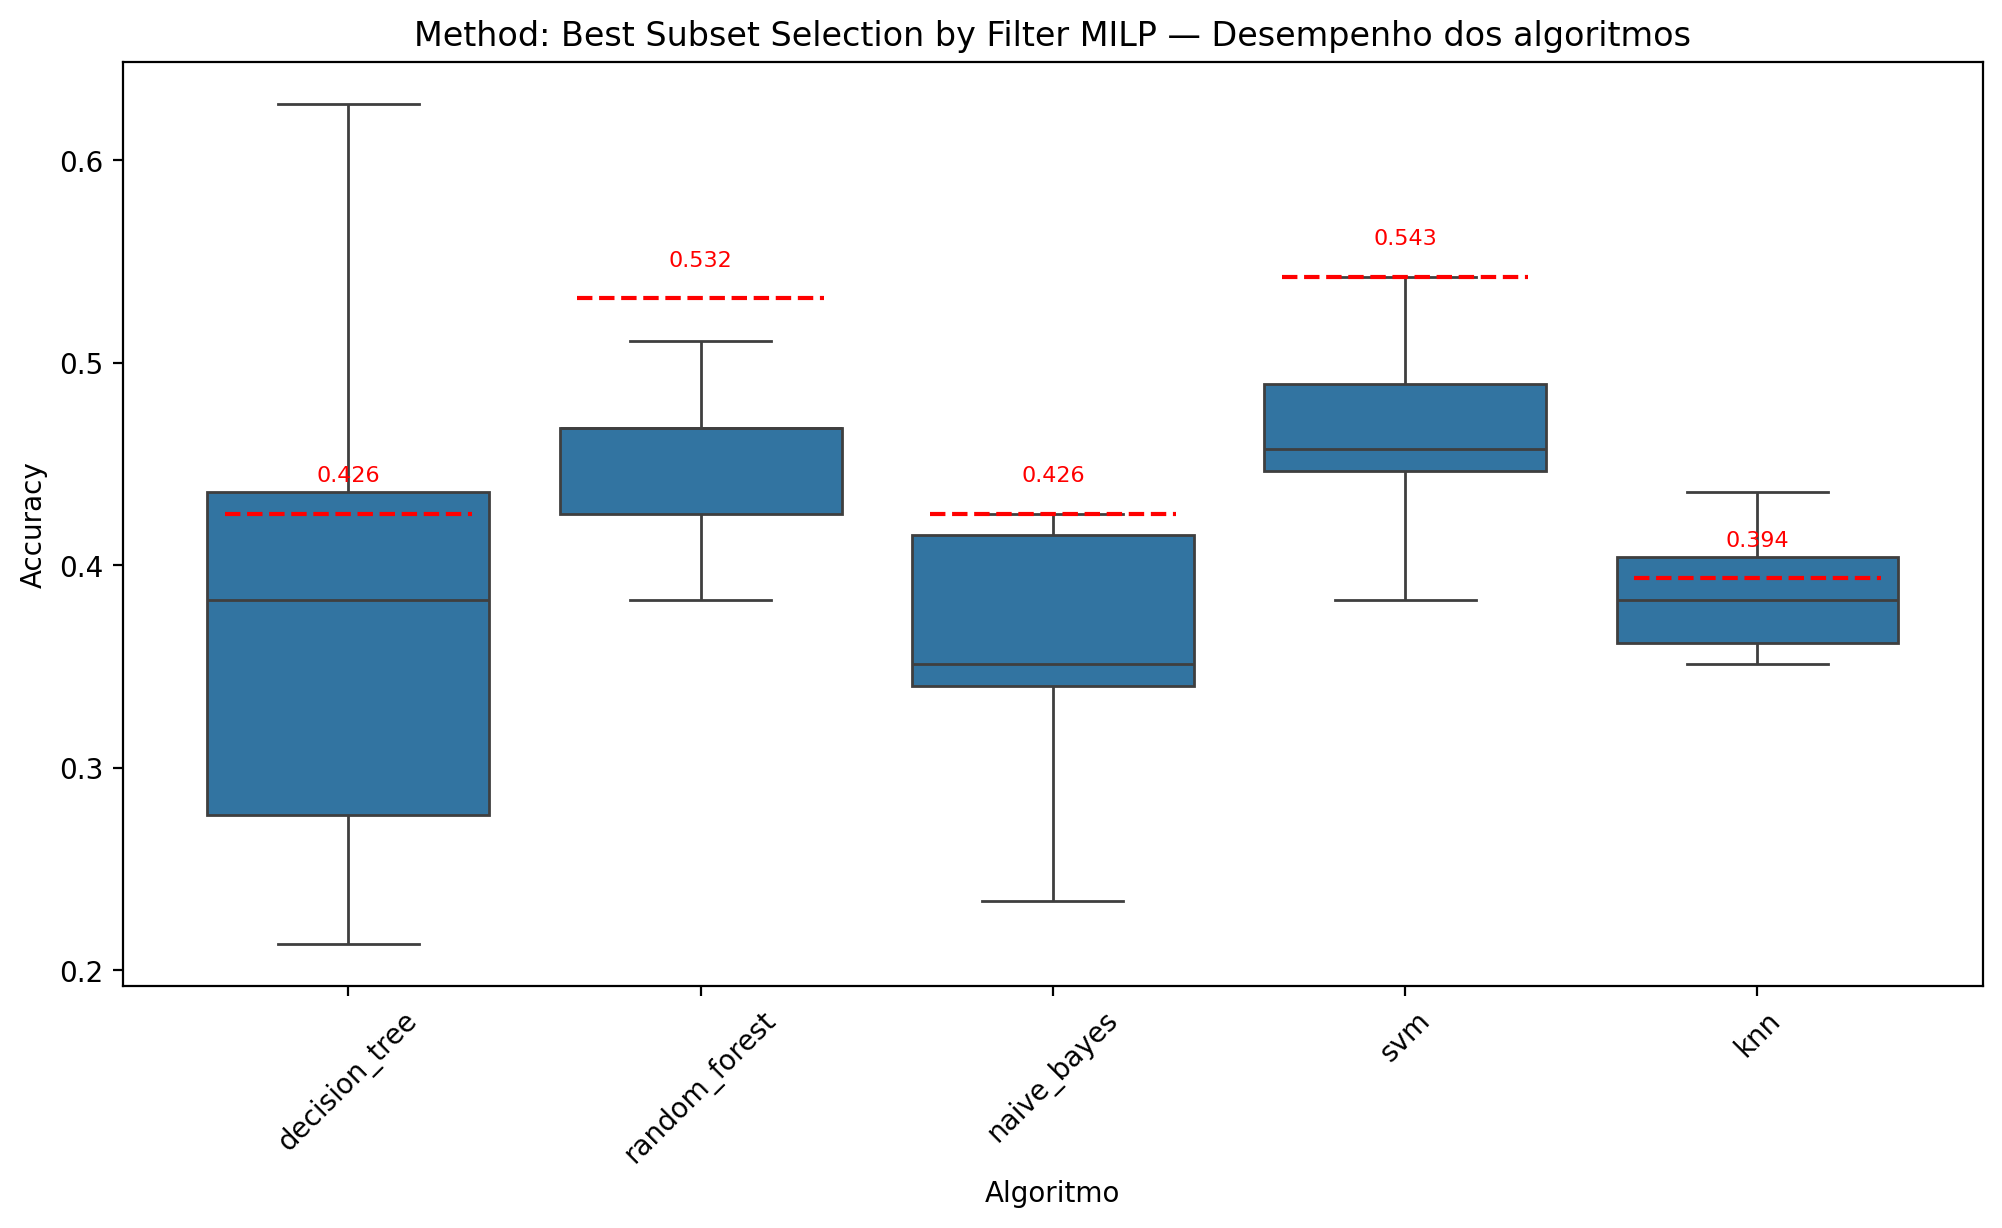
\includegraphics[width=.32\textwidth]{boxplot_method_Best_Subset_Selection_by_Filter_MILP.png}
\hfill
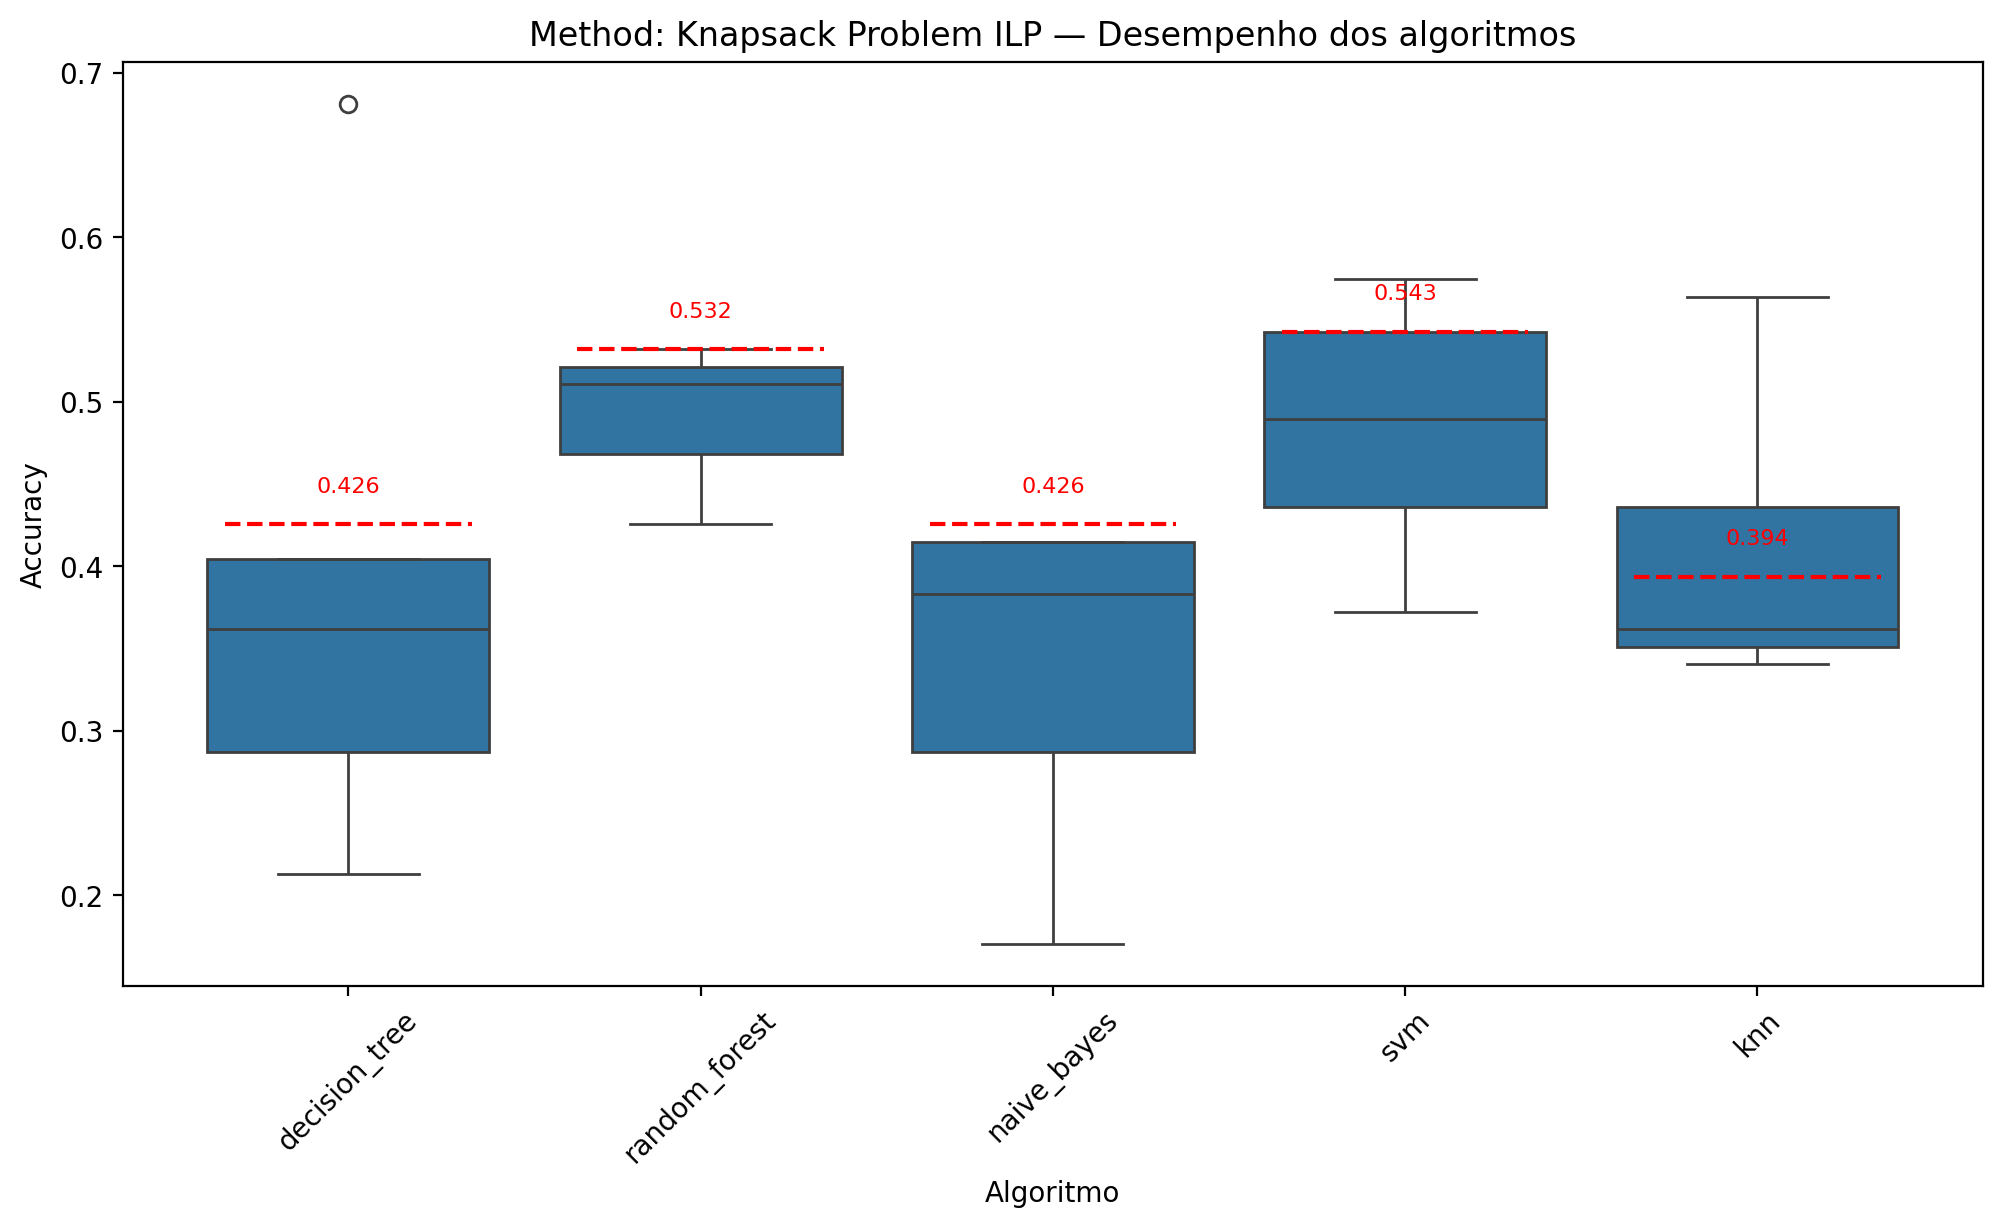
\includegraphics[width=.32\textwidth]{boxplot_method_Knapsack_Problem_ILP.png}
\hfill
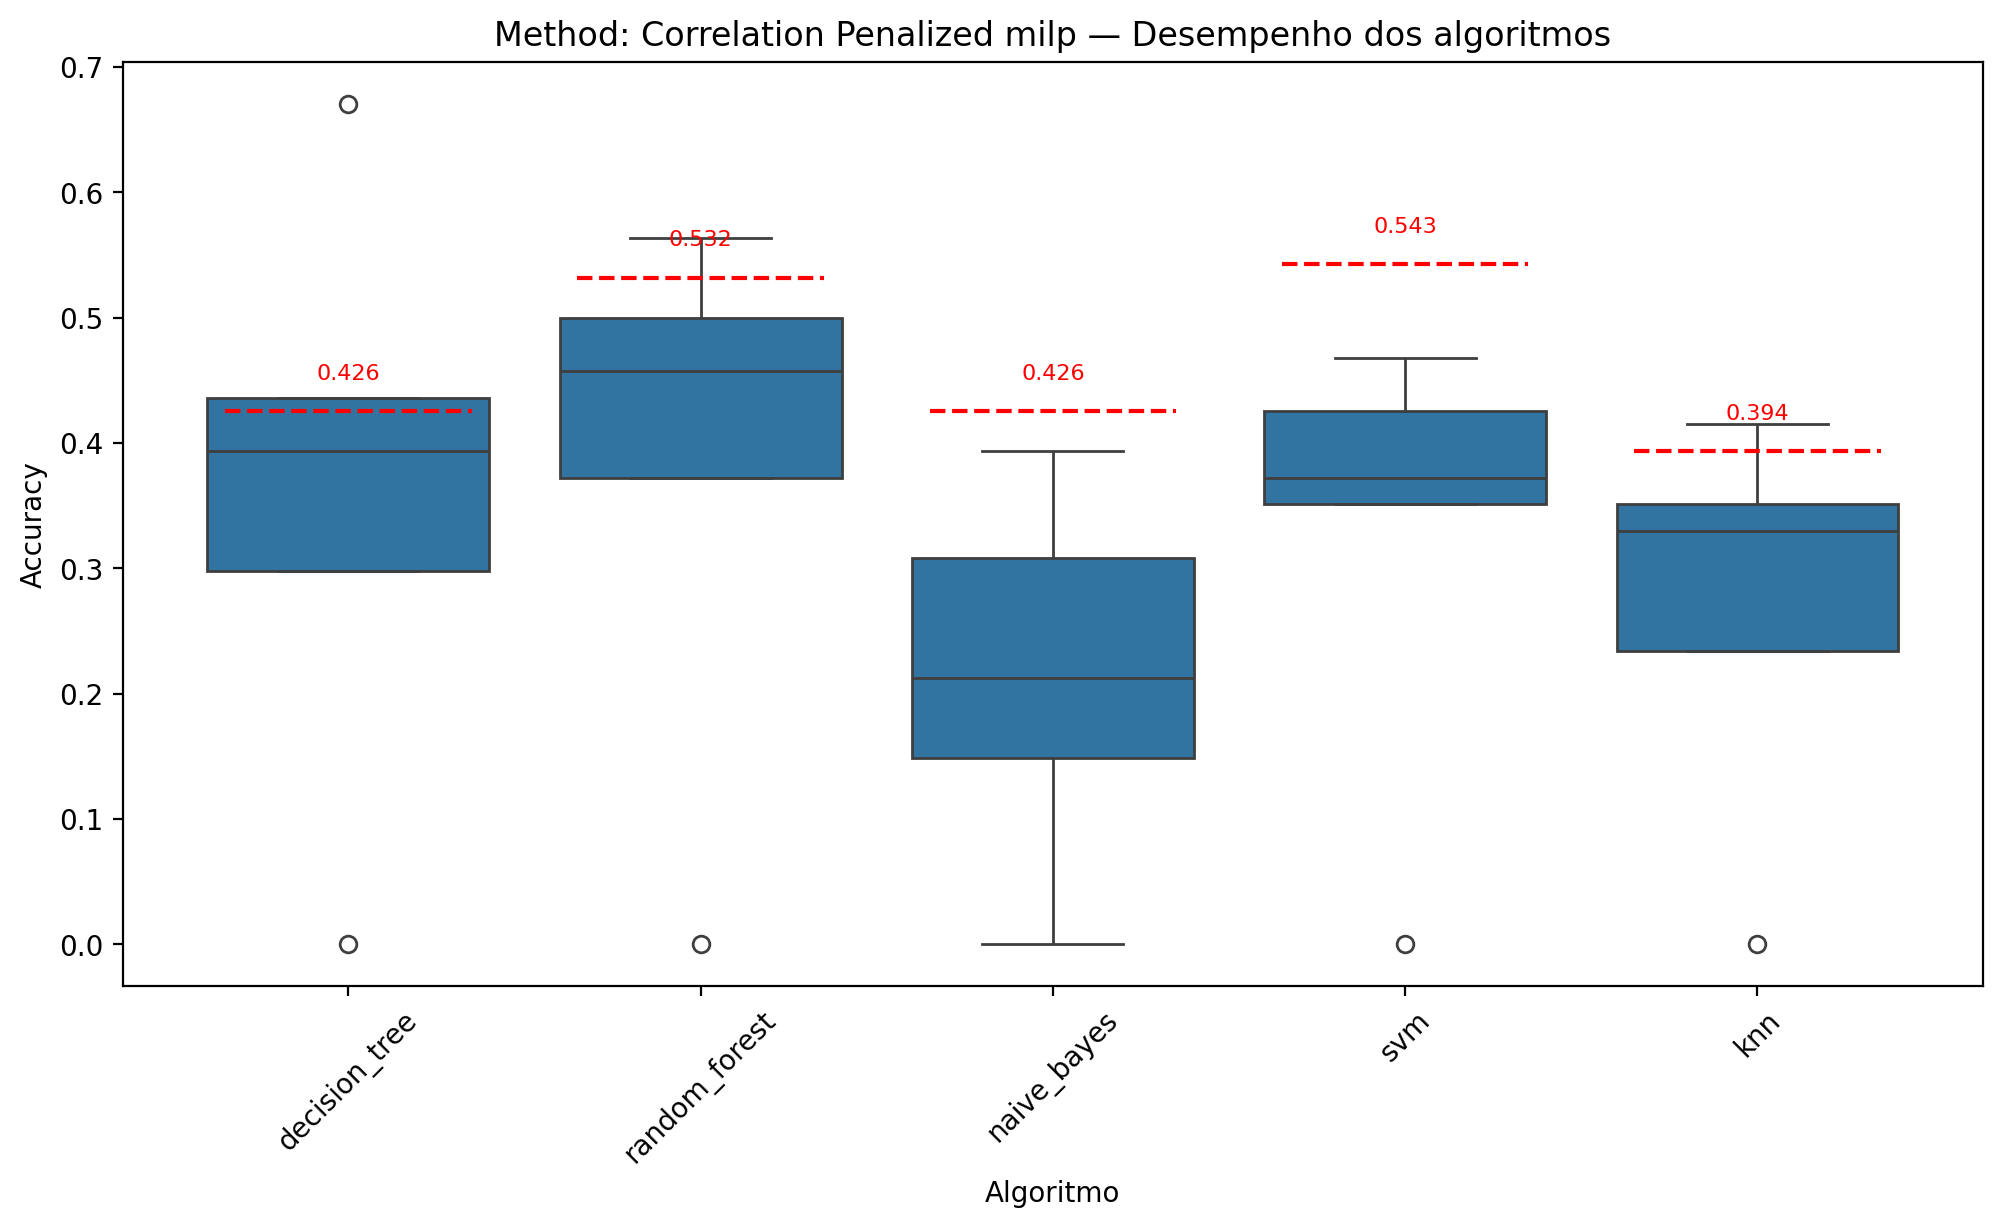
\includegraphics[width=.32\textwidth]{boxplot_method_Correlation_Penalized_milp.png}
\caption{Desempenho dos algoritmos utilizando as modelagens de métodos exatos para seleção de meta-features.}
\label{fig:boxplots_exatos}
\end{figure}

Como está sendo tratado um problema de categorização, é normal que algoritmos de natureza categórica, como DecisionTree e RandomForest, tenham um desempenho melhor que os outros, pois eles conseguem delimitar melhor o espaço de busca e as características que separam os datasets.

\begin{table}[ht]
\centering
\caption{Acurácia média obtida no nível meta a partir da seleção por métodos exatos.}
\label{tab:metodos_exatos}
\begin{tabular}{llcc}
\hline
\textbf{Método} & \textbf{Melhor Algoritmo} & \textbf{Acurácia Média} & \textbf{Meta-features} \\
\hline
Melhor Subset & Decision Tree & 0.6276 & 200 \\
Knapsack com Penalidade & Decision Tree & 0.6808 & 23 \\
Knapsack Quadratica & Decision Tree & 0.6702 & 17 \\
\hline
\end{tabular}
\end{table}

Com isso, observando a Tabela~\ref{tab:metodos_exatos}, nota-se que em nível meta o algoritmo DecisionTree foi o responsável por obter o melhor desempenho (acurácia de 62,76\%). Além disso, a filtragem inicial reduziu drasticamente o espaço de mais de 1000 atributos para um conjunto refinado de 66 características. Isso impacta positivamente de forma direta tanto o custo de treinamento quanto a velocidade do modelo final na predição. Esses achados corroboram estudos empíricos anteriores na literatura \cite{pereira2021evaluating}, que também demonstraram que abordagens de seleção de meta-features e redução de dimensionalidade conseguem descartar grande parte das características originais mantendo a performance e acelerando consideravelmente o tempo de execução.

\subsection{Métodos Aproximados}

A Tabela~\ref{tab} apresenta os resultados obtidos com as três variações de Algoritmo Genético testadas neste trabalho. Esses resultados estão relacionados ao desempenho no nível meta, ou seja, à capacidade do meta-modelo de indicar qual algoritmo de aprendizado de máquina tende a apresentar melhor desempenho para uma determinada base de dados, utilizando apenas as meta-features selecionadas por cada abordagem.

\begin{table}[ht]
\centering
\caption{Comparação dos algoritmos genéticos para seleção de meta-features.}
\label{tab}
\begin{tabular}{lcccc}
\hline
\textbf{Método} & \textbf{Acurácia média} & \textbf{Desvio} & \textbf{Fitness} & \textbf{Meta-features} \\
\hline
AG 1 -- Clássico binário & 0,6339 & 0,0542 & 0,6150 & 66 \\
AG 2 -- Guiado por MI + busca local & 0,6866 & 0,0700 & 0,6684 & 31 \\
AG 3 -- Compacto/esparso & 0,6661 & 0,0723 & 0,6507 & 18 \\
\hline
\end{tabular}
\end{table}

Observando os resultados, percebe-se que o AG 1 foi o método que selecionou a maior quantidade de meta-features, com 66 atributos escolhidos entre os 150 disponíveis após a etapa de filtragem. Isso representa cerca de 44\% do conjunto final de atributos. Apesar de ter apresentado o menor desvio-padrão entre os três métodos, ele obteve a menor acurácia média. Esse resultado mostra que selecionar mais atributos não significa, necessariamente, melhorar o desempenho do meta-modelo. Nesse caso, o AG clássico acabou mantendo um subconjunto maior, mas sem conseguir superar as outras abordagens.

O AG 2 foi o método com melhor desempenho geral. Ele alcançou acurácia média de 0,6866, utilizando 31 meta-features. Esse resultado indica que o uso da Mutual Information para orientar a inicialização da população, junto com a etapa de busca local, ajudou o algoritmo a encontrar subconjuntos mais relevantes. Além disso, o método conseguiu reduzir bastante a quantidade de atributos em relação ao AG 1, mantendo o melhor valor de fitness entre as três abordagens.

Já o AG 3 selecionou o menor subconjunto de meta-features, com apenas 18 atributos. Mesmo utilizando uma quantidade bem menor de características, ele obteve acurácia média de 0,6661, ficando abaixo do AG 2, mas ainda acima do AG 1. Esse resultado é interessante porque mostra que uma solução mais compacta ainda pode manter um desempenho competitivo. Dessa forma, o AG 3 se destaca quando o objetivo é reduzir ao máximo a quantidade de atributos, mesmo que isso gere uma pequena perda de acurácia em comparação com o melhor resultado.

As Figuras~\ref{fig} e~\ref{fig} apresentam, respectivamente, a evolução da acurácia média e da quantidade de meta-features selecionadas ao longo das gerações. Esses gráficos ajudam a visualizar como cada algoritmo evoluiu durante a busca e como ocorreu o equilíbrio entre desempenho e redução do número de atributos.

\begin{figure}[ht]
\centering
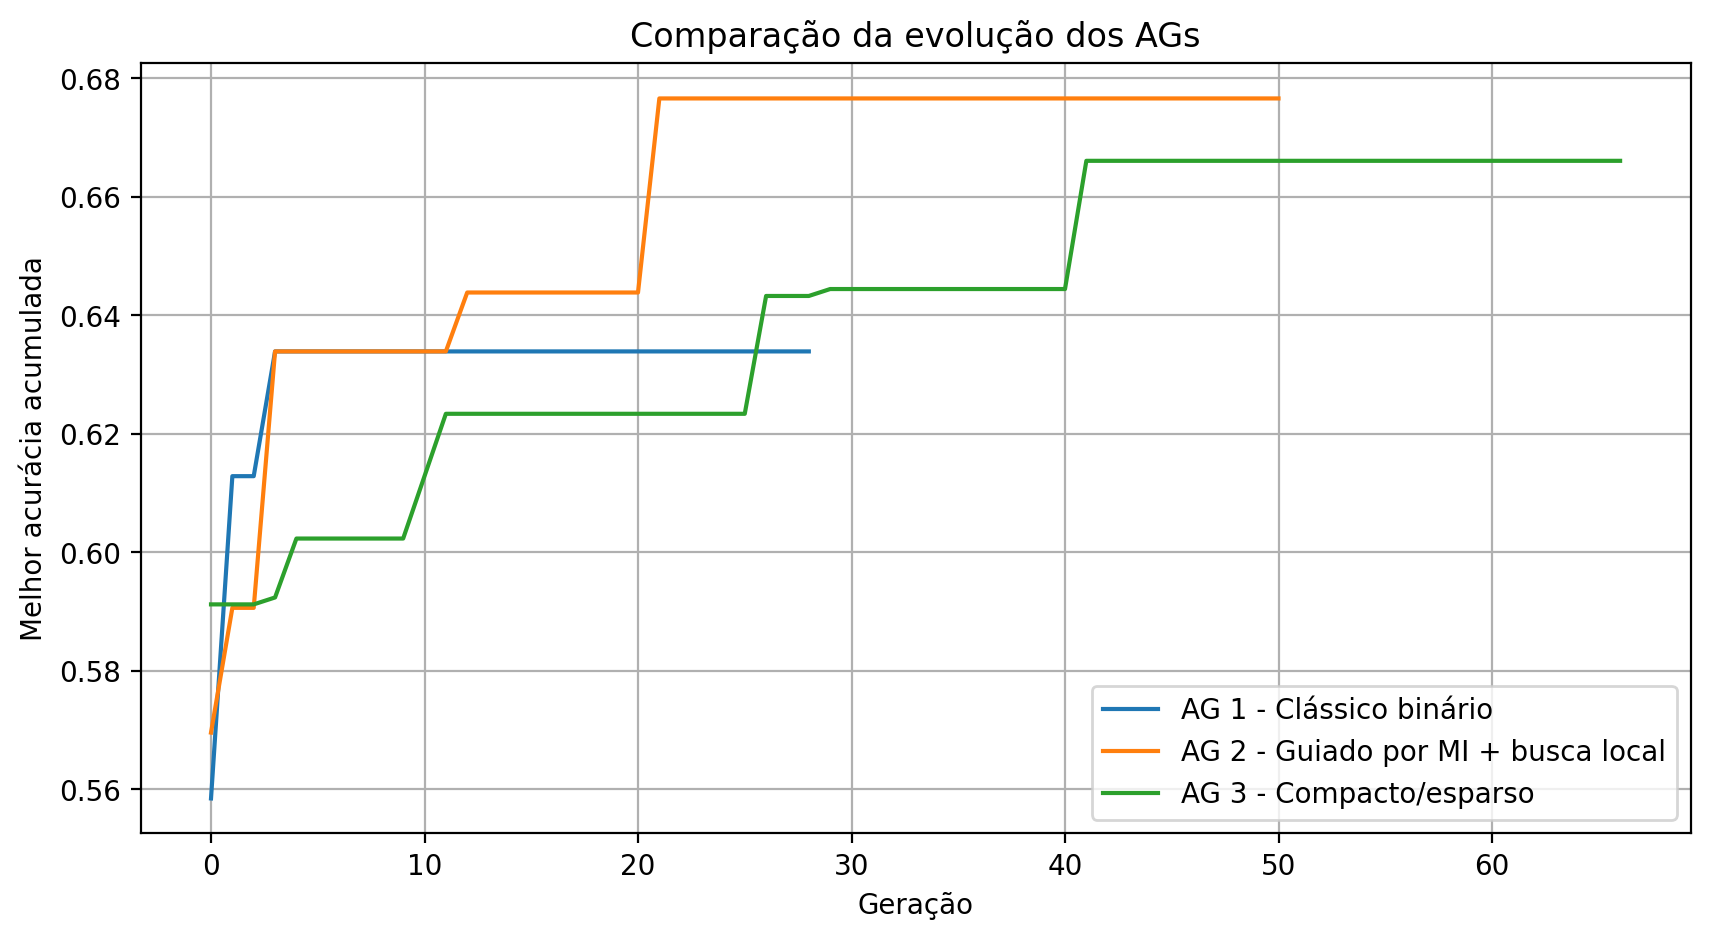
\includegraphics[width=.85\textwidth]{evolution_ag_accuracy.png}
\caption{Evolução da melhor acurácia média acumulada dos algoritmos genéticos.}
\label{fig}
\end{figure}

\begin{figure}[ht]
\centering
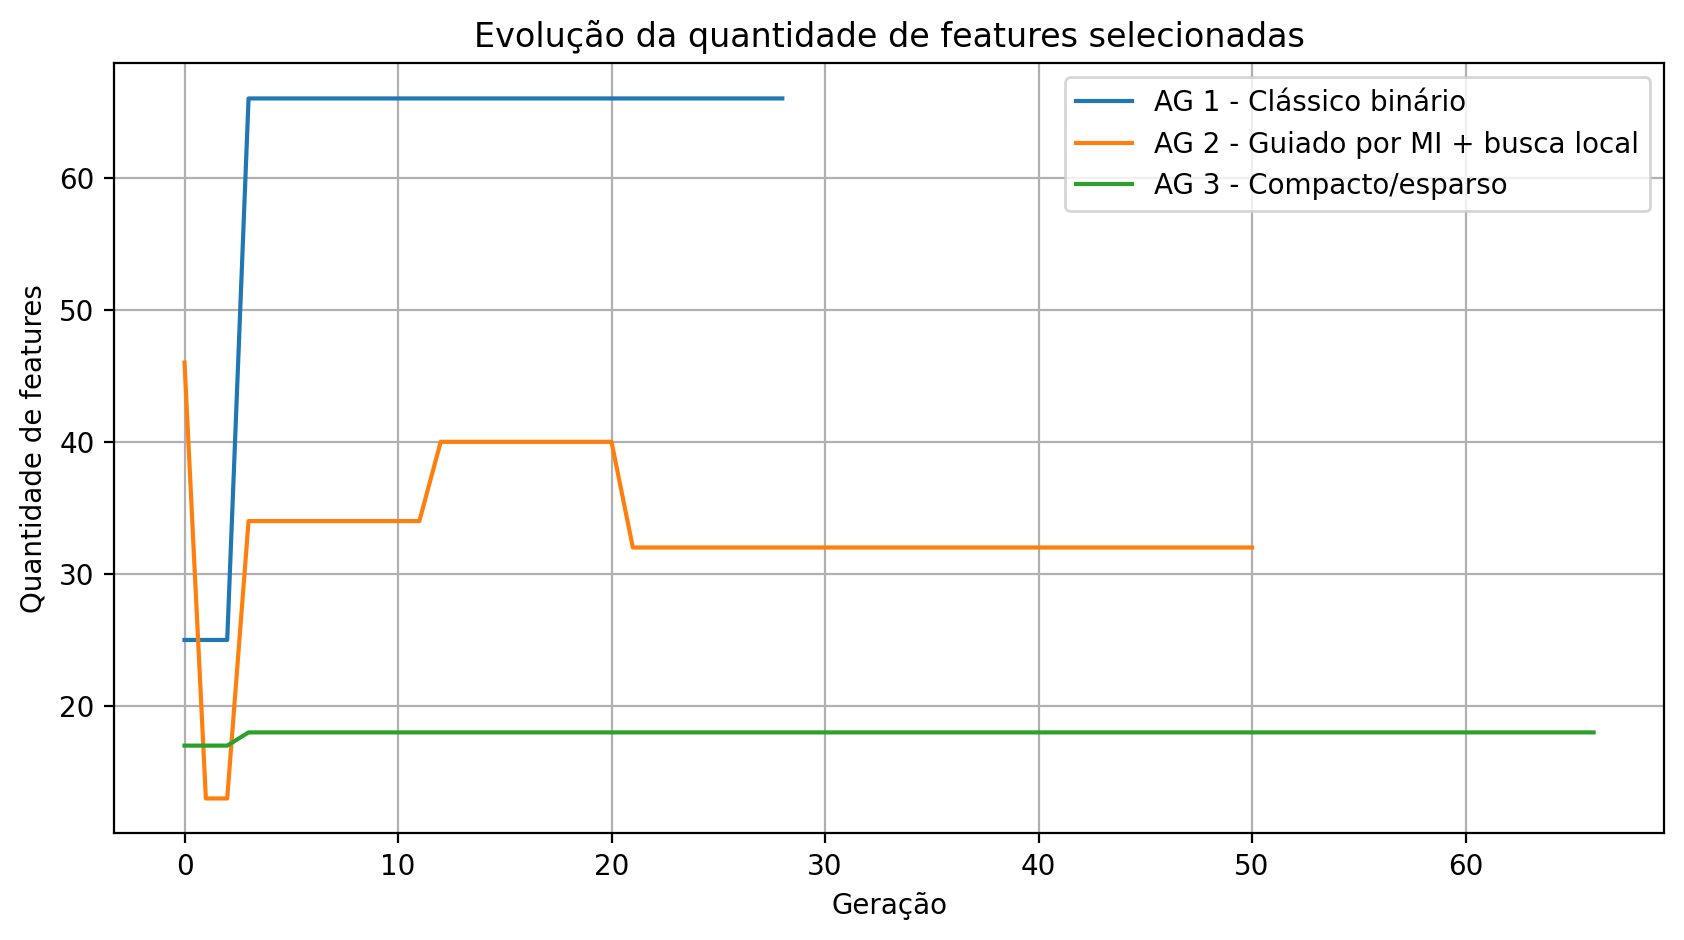
\includegraphics[width=.85\textwidth]{evolution_ag_n_features.png}
\caption{Evolução da quantidade de meta-features selecionadas pelos algoritmos genéticos.}
\label{fig}
\end{figure}

De modo geral, os resultados mostram que o AG 2 foi a melhor opção quando o foco principal é obter maior acurácia no meta-modelo. Por outro lado, o AG 3 foi o mais eficiente em termos de redução dimensional, pois selecionou o menor conjunto de meta-features e ainda manteve um desempenho próximo ao melhor resultado. O AG 1 serviu como uma boa base de comparação, mas foi menos eficiente, já que selecionou mais atributos e apresentou menor acurácia.

\subsection{Abordagem Híbrida}

Com um pré-processamento reduzindo bastante as meta-features iniciais e direcionando uma população elitista com as melhores combinações matemáticas, a abordagem híbrida elevou significativamente o desempenho em relação aos outros métodos puramente aproximados. Entretanto, o número de gerações necessárias para a convergência e a estabilização do algoritmo oscilaram consideravelmente, como ilustra a Figura~\ref{fig:hybrid_n_features}. Isso impacta de forma direta o tempo de processamento necessário para selecionar e refinar os atributos na criação do meta-modelo.

\begin{figure}[ht]
\centering
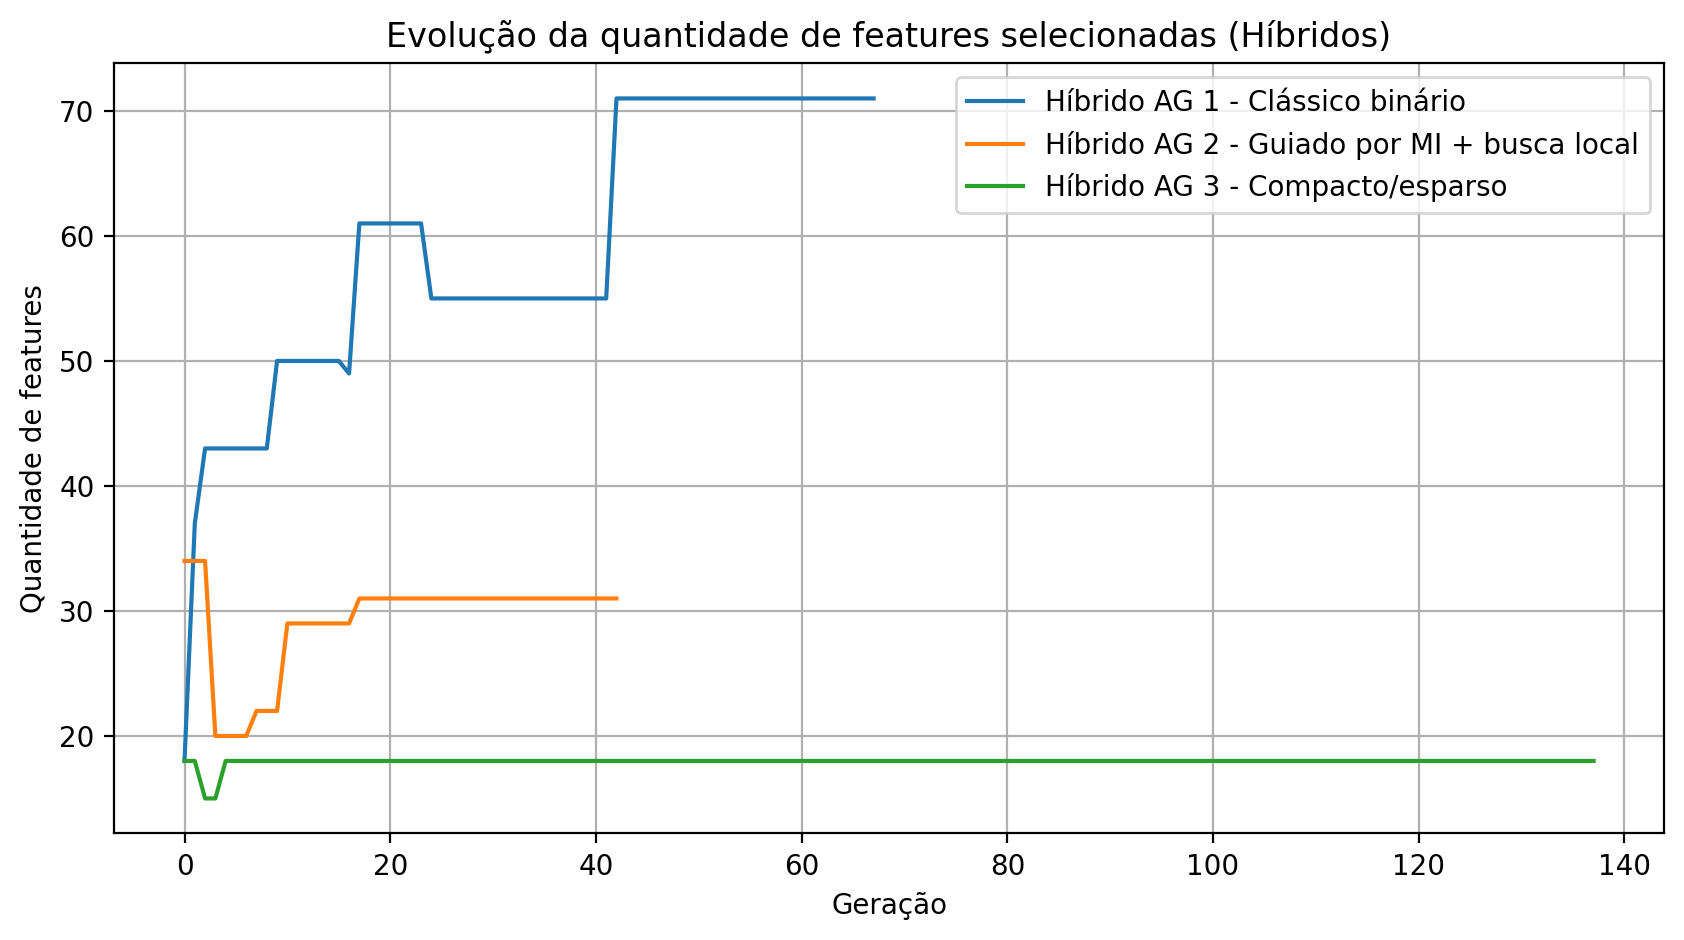
\includegraphics[width=.85\textwidth]{evolution_ag_hybrid_n_features.png}
\caption{Evolução da quantidade de meta-features selecionadas durante a abordagem híbrida.}
\label{fig:hybrid_n_features}
\end{figure}

Porém, a abordagem híbrida se destacou substancialmente na acurácia geral. Os meta-modelos obtiveram um salto de desempenho contínuo ao longo das gerações, indicando o sucesso do escape de ótimos locais, como demonstrado na Figura~\ref{fig:hybrid_accuracy}. Esse avanço traduz-se em uma maior precisão recomendatória, repercutindo beneficamente não apenas no nível meta, mas, por consequência, na escolha assertiva do algoritmo de nível base.

\begin{figure}[ht]
\centering
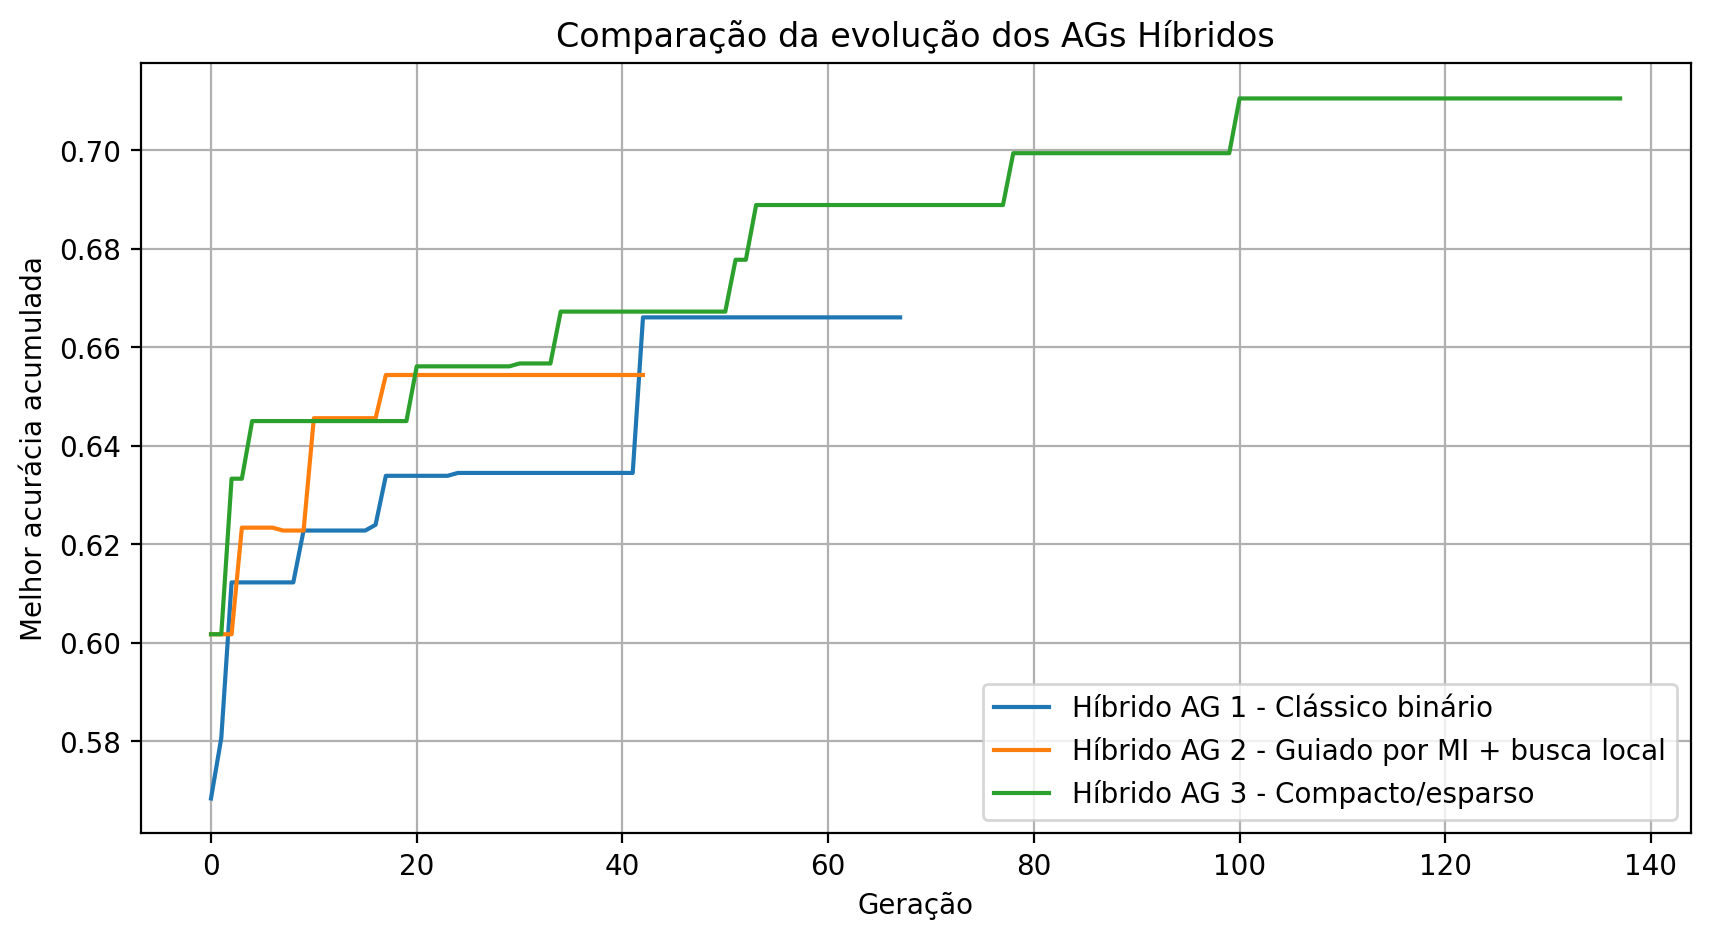
\includegraphics[width=.85\textwidth]{evolution_ag_hybrid_accuracy.png}
\caption{Evolução da melhor acurácia média acumulada na abordagem híbrida.}
\label{fig:hybrid_accuracy}
\end{figure}

Por fim, a Tabela~\ref{tab:hybrid} descreve a comparação quantitativa exata das três formulações testadas para a abordagem híbrida, destacando a acurácia média e a quantidade de meta-features finais do melhor indivíduo.

\begin{table}[ht]
\centering
\caption{Comparação final das variações da abordagem híbrida.}
\label{tab:hybrid}
\begin{tabular}{lcccc}
\hline
\textbf{Método} & \textbf{Acurácia média} & \textbf{Desvio} & \textbf{Fitness} & \textbf{Meta-features} \\
\hline
Híbrido AG 1 - Clássico binário & 0,6660 & 0,1037 & 0,6433 & 71 \\
Híbrido AG 2 - Guiado (MI) & 0,6649 & 0,1084 & 0,6433 & 30 \\
Híbrido AG 3 - Compacto/esparso & 0,7105 & 0,0954 & 0,6924 & 18 \\
\hline
\end{tabular}
\end{table}

Destaca-se que o Híbrido AG 3 (Compacto/Esparso) conseguiu uma acurácia superior (71,05\%) exigindo impressionantes 18 meta-features, configurando a melhor relação de custo e precisão preditiva de toda a experimentação. No entanto, o principal ponto negativo da abordagem híbrida continua sendo sua complexidade de execução sequencial e o extenso custo computacional. Em contextos ou cenários industriais nos quais se exige um re-treinamento rápido e dinâmico, talvez não seja a alternativa mais pragmática.

\subsection{Discussão geral}

Os resultados sintetizados evidenciam que, ao comparar globalmente a performance em nível base com a performance do nível meta (Figuras~\ref{fig:acc_base} e~\ref{fig:acc_meta}), a escolha informada do pipeline de machine learning se mostra muito superior às abordagens estáticas ou triviais. Observamos que os desempenhos individuais dos classificadores em nível base tendem a oscilar significativamente de acordo com a complexidade e a natureza topológica do dataset, reforçando a premissa de que não existe um "algoritmo universal" que triunfe em todos os cenários. 

\begin{figure}[ht]
\centering
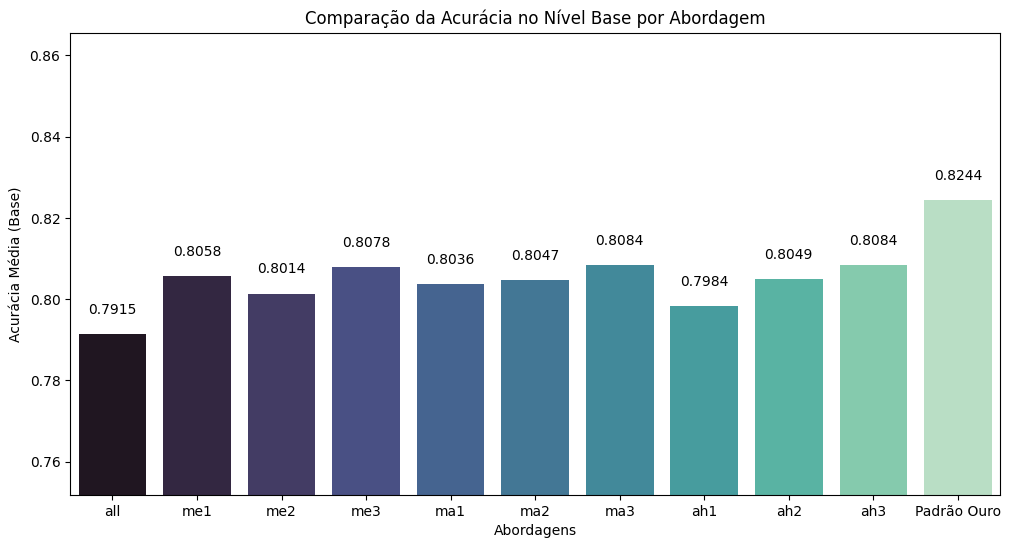
\includegraphics[width=.85\textwidth]{acc_base.png}
\caption{Acurácia média isolada dos classificadores no nível base para os datasets.}
\label{fig:acc_base}
\end{figure}

Quando a seleção de algoritmos é governada pelo meta-aprendizado de características (nível meta), a performance geral do sistema atinge estabilidade e os piores cenários (onde modelos fracassariam miseravelmente por incapacidade algorítmica) são mitigados pela recomendação ativa de modelos mais propensos a capturar o padrão adjacente dos dados.

\begin{figure}[ht]
\centering
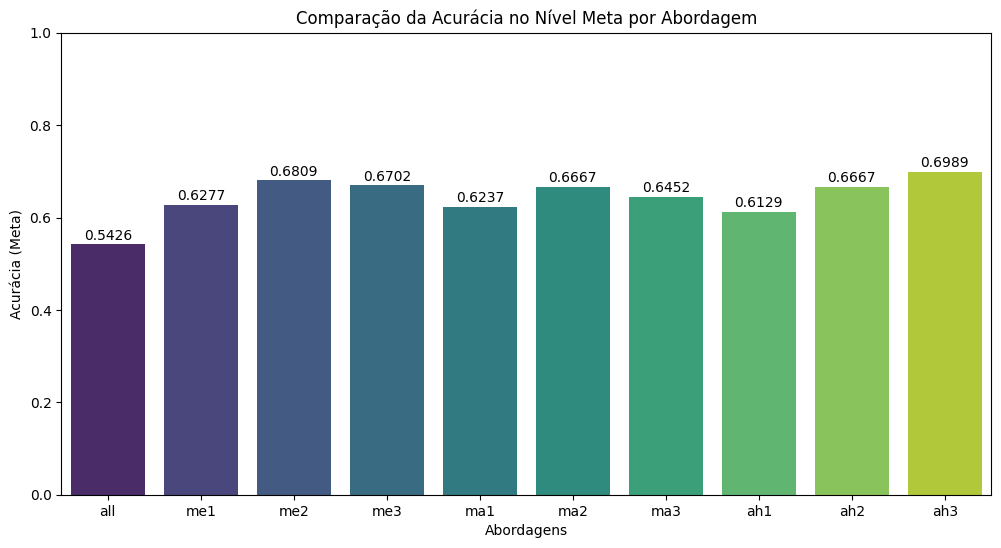
\includegraphics[width=.85\textwidth]{acc_meta.png}
\caption{Melhoria da acurácia e estabilização de resultados conduzida pelo sistema de nível meta.}
\label{fig:acc_meta}
\end{figure}

\section{Conclusão}

O problema de recomendação de algoritmos no contexto de meta-aprendizado não diz respeito apenas a prever o modelo de melhor acurácia, mas a entender qual parte da informação do dado tem poder preditivo e qual parte só causa "ruído". Como demonstrado, as ferramentas modernas extraem facilmente milhares de meta-features dos datasets. Contudo, arrastar toda essa dimensionalidade pelo fluxo de Machine Learning acarreta lentidão, sobreajuste (overfitting) e imensa confusão estatística para os meta-modelos. Isso é demonstrado quando houve extração das caracteristicas com pymfe e treinando sem o refinamento da seleção.

Ao investigar diferentes arquiteturas — passando pelos métodos exatos, explorando as heurísticas aproximativas com Algoritmos Genéticos (AG) e combinando forças em uma abordagem híbrida, observamos comportamentos que evidenciam trade-offs muito claros da engenharia de software e pesquisa operacional.

Os \textbf{métodos exatos} demonstraram que modelagens matemáticas (como a formulação do Problema da Mochila com Penalidade ou Penalização por Correlação -Problema da Mochila Quadratica -) garantem recortes robustos do espaço dimensional. Ao limitar o meta-modelo (como a Decision Tree) a utilizar apenas os 66 atributos mais valiosos, o tempo de inferência caiu abruptamente e o "ruído" foi podado com garantias lineares. 

Os \textbf{métodos aproximados (Algoritmos Genéticos)} provaram que não é preciso inspecionar todo o espaço exaustivo. Especificamente, a variação que atrelou a inicialização estocástica ao conhecimento prévio de Information Gain (Mutual Information) ofereceu um equilíbrio brilhante. O AG conseguiu pinçar atributos que, combinados de forma não-linear, subiram o nível do jogo e entregaram desempenhos superiores.

No entanto, foi na \textbf{abordagem híbrida (Seeded GA)} que obtivemos as respostas mais contundentes para o limite tecnológico do estudo. Injetar soluções exatas como "elites" iniciais na evolução heurística guiou o AG a espaços de busca profundos, descobrindo que utilizar apenas \textbf{18 meta-features} gerava impressionantes 71,05\% de assertividade no nível meta, porém ao treinar novamente o dataset não necessáriamente chegou-se aos 71,05\%. Isso traduz um achado expressivo: menos de 2\% do escopo de características inicial é suficiente para predizer adequadamente o comportamento de múltiplos algoritmos de aprendizado de máquina, quando essa seleção é cirúrgica e otimizada.

A contrapartida dessa excelência, porém, reside no alto custo processual dessa hibridização. Treinar, extrair, penalizar de forma exata e só então evoluir geneticamente as populações pode não ser viável para sistemas baseados em velocidade. Como alternativa ao gargalo provocado pelo retreinamento constante, estudos recentes propõem abstrações inovadoras que transformam o espaço de busca discreto em contínuo utilizando meta-aprendizado \cite{metafs2023}, o que fortalece a justificativa do limite técnico enfrentado no presente estudo empírico. O verdadeiro valor deste estudo encontra-se justamente neste discernimento: para pipelines que necessitam de extração e de baixo atrito, métodos de filtragem diretos ou genéticos esparsos são recomendados. Todavia, para sistemas massivos e estáveis de recomendação acadêmica e de Auto-ML, gastar o peso computacional na fase híbrida irá pavimentar, invariavelmente, os melhores e mais enxutos caminhos para as inferências base.

\bibliographystyle{sbc}
\bibliography{sbc-template}

\end{document}

